\documentclass[12pt]{phage3slides} %

\beamertemplatenavigationsymbolsempty

\logo{
\includegraphics[width=1.4cm]{gga-small.png}}
\title[Galaxy for Genome Annotation, Teaching, Databases]{GGA: Galaxy for Genome Annotation, Teaching, and Genomic Databases}
\author[ER, BG, ND, AB]{Eric Rasche, Bj\"orn Gr\"uning, Nathan Dunn, Anthony Bretaudeau}
\date{2017-06-29T09:50:00Z}

\begin{document}
\frame{\titlepage}

% GMOD projects have long provided powerful open-source tools to the
% bioinformatics community, but have historically been hard to configure
% and integrate. The Galaxy Genome Annotation (GGA) group provides a
% highly integrated set of Dockerized GMOD projects allowing for more
% widespread use of these tools in new contexts for system
% administrators wishing to deploy the suite. Our projects include
% maintenance of the Galaxy-Apollo bridge tools, Galaxy-Tripal and Chado
% tooling, and containerized versions of various GMOD projects which are
% configured to easily integrate with the rest of the suite.

% This talk will explore the use of this suite in the context of a real
% life use-case, an undergraduate phage annotation course. We will cover
% the GGA suite as well as various integrations, workflows, training
% materials, and tools that were built and made available in support of
% GGA.

% Very interesting subject. We encourage the presenters to focus on 3-4 key
% aspects of the project rather than try to cover every aspect.

\section[GGA]{Galaxy for Genome Annotoation}
\begin{frame}{Galaxy for Genome Annotation}
    Galaxy is great for:
    \begin{itemize}
        \item NGS Analysis
        \item Assembly
        \item ...
        \item Annotation Analysis (Tabular processing, etc)
        \item *omics
    \end{itemize}
    But we are missing the Annotation step.\\\ \\
    We are missing the tooling, the
    trainings, and the community for genome annotation.
\end{frame}

\subsection{What}
\begin{frame}{What are we building?}
    \begin{columns}
        \begin{column}{0.38\textwidth}
            \begin{itemize}
                \item Galaxy Flavour(s)
                \item GMOD Containers
                \item Glue Code
                \item Training Materials
                \item Peripherals
                \item Community
                \item Tools
            \end{itemize}
        \end{column}
        \begin{column}{0.58\textwidth}
            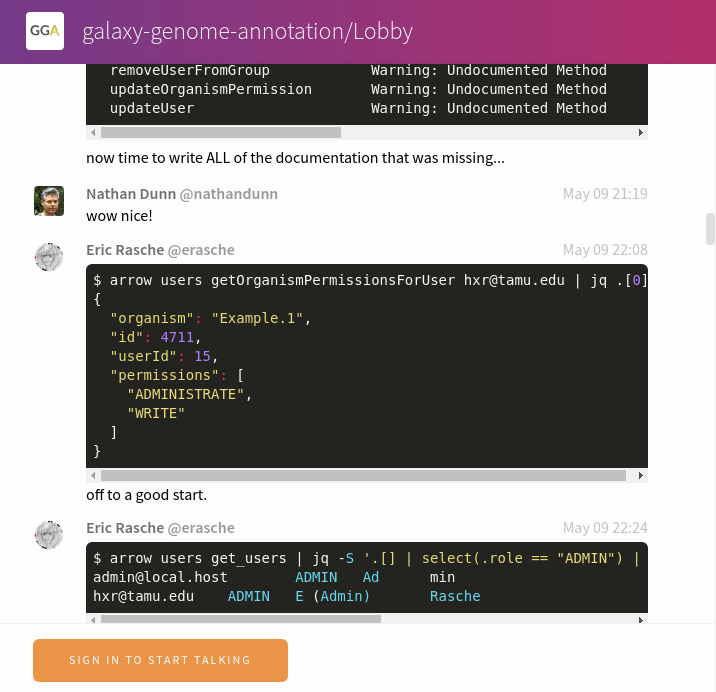
\includegraphics[width=3cm]{img/gga-chat.png}
            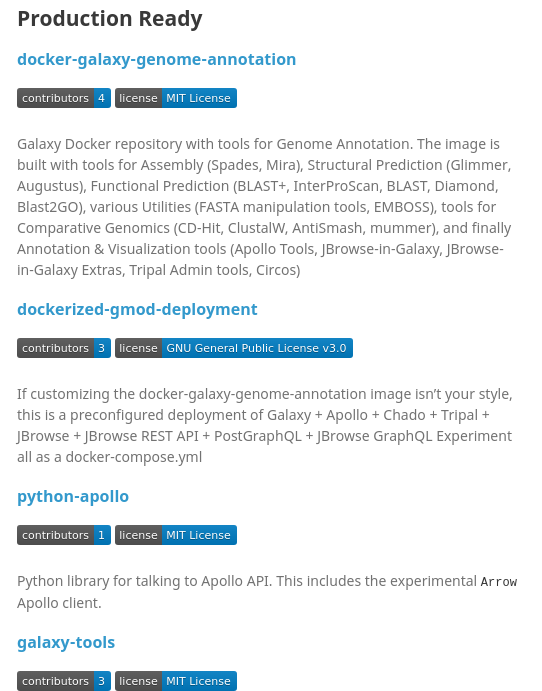
\includegraphics[width=3cm]{img/gga-gh.png} \\[.7cm]
            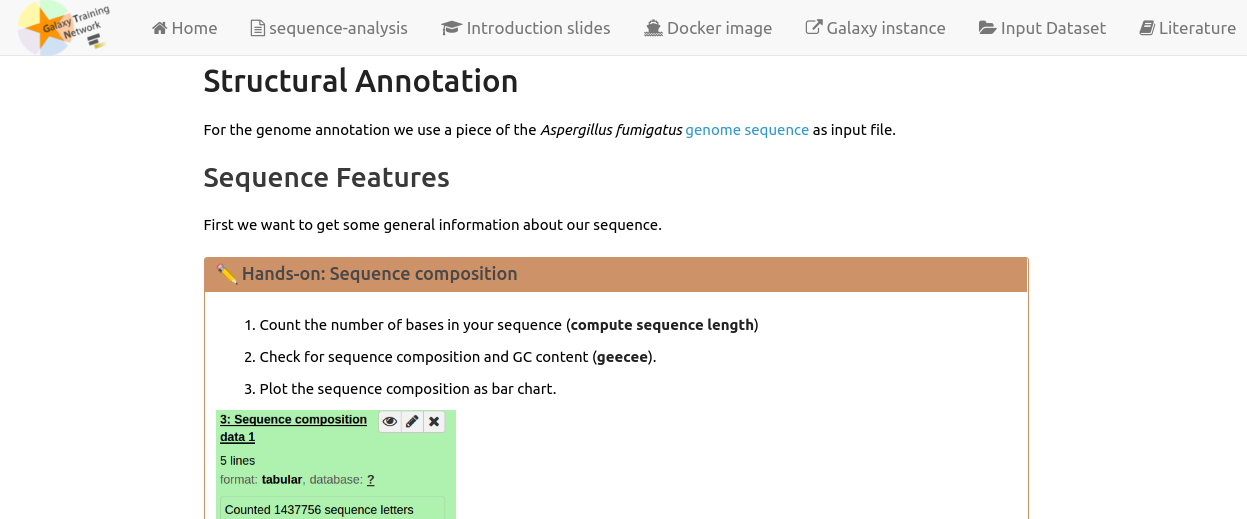
\includegraphics[width=6cm]{img/gga-docs.png}
        \end{column}
    \end{columns}
\end{frame}

\subsection{Who}
\begin{frame}{Who are we?}
    \begin{columns}
        \begin{column}{0.48\textwidth}
            \begin{itemize}
                \item CPT Phage Team (Eric Rasche, Eleni Mijalis, Cory Maughmer)
                \item Anthony Bretaudeau
                \item Nathan Dunn
                \item Bj\"orn Gr\"uning
                \item Peter van Heusen
                \item Suzanna Lewis
                \item Eduardo de Paiva Alves
                \item Torsten Seemann
                \item (\ldots you!)
            \end{itemize}
        \end{column}
        \begin{column}{0.48\textwidth}
            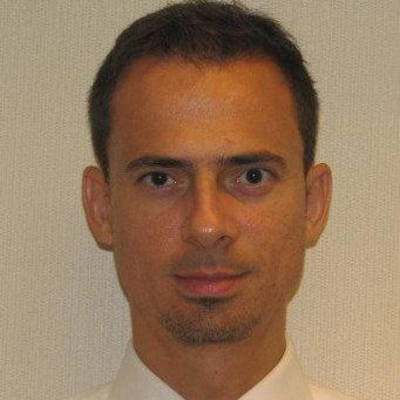
\includegraphics[width=1.5cm]{people/Eduardo-Alves}
            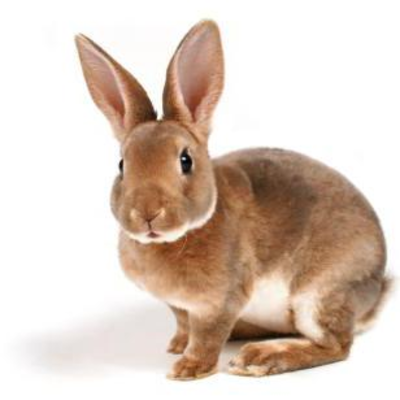
\includegraphics[width=1.5cm]{people/abretaud}
            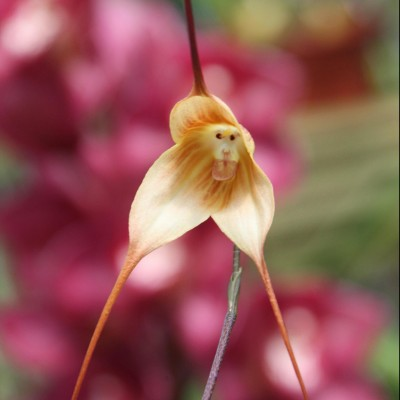
\includegraphics[width=1.5cm]{people/bgruening} \\
            
\includegraphics[width=1.5cm]{people/elenimijalis}
            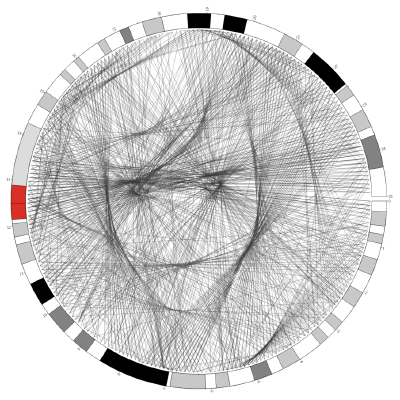
\includegraphics[width=1.5cm]{people/erasche}
            
\includegraphics[width=1.5cm]{people/moffmade} \\
            
\includegraphics[width=1.5cm]{people/selewis}
            
\includegraphics[width=1.5cm]{people/nathandunn}
            
\includegraphics[width=1.5cm]{people/pvanheus} \\
            
\includegraphics[width=1.5cm]{people/tseemann}
        \end{column}
    \end{columns}
\end{frame}

\subsection{Why}
\begin{frame}{Why?}
    \begin{itemize}
        \item GMOD at its best
        \item Annotation still requires humans
        \item Powerful Analysis + Interactive Annotations
        %\item Fun Challenges
        \item Useful to real-life people, solve real problems
        \item Project longevity
    \end{itemize}
\end{frame}





\section{Infrastructure}
\begin{frame}{\#InfrastructureGoals}
    \begin{center}
        
\includegraphics[scale=0.2]{img/launch} \\
        
\includegraphics[scale=0.2]{img/share} \\
        
\includegraphics[scale=0.2]{img/customize} \\
    \end{center}
\end{frame}

\subsection{Solutions}
\begin{frame}{Infrastructure Solutions}
    \begin{itemize}
        \item Docker Image: Galaxy + Annotation Tools {\color{gray}(Apollo Tools, Tripal Admin Tools, Circos, JBrowse, BLAST+, InterProScan, Glimmer, Augustus, FASTA manipulation tools, Spades, Mira, CD-Hit, ClustalW, AntiSmash, mummer, EMBOSS, BLAST, Diamond, Blast2GO, \ldots{})}
        \item Dockerized GMOD Deployment {\color{gray}(Galaxy, JBrowse, Apollo, Chado, Chado APIs, Tripal pre-configured to work together seamlessly)}
        \item Apollo, Chado python libraries {\color{gray}(+parsec like tools, ``Arrow'' and ``Chakin'')}
        \item Various Apollo support projects {\color{gray}(git-backup, experimental google docs integration)}
    \end{itemize}
\end{frame}

\subsection{Galaxy-Apollo}
\begin{frame}{Galaxy / Apollo Bridge}
    \begin{columns}
        \begin{column}{0.58\textwidth}
            \begin{itemize}
                %\item Grew out of use in an undergraduate course
                \item Initially quite simple, only a tool to add an organism (JBrowse instance) to Apollo
                \item Now includes automation (tools for creating/editing annotations)
                \item Tested and revised in collaboration with curators
            \end{itemize}
            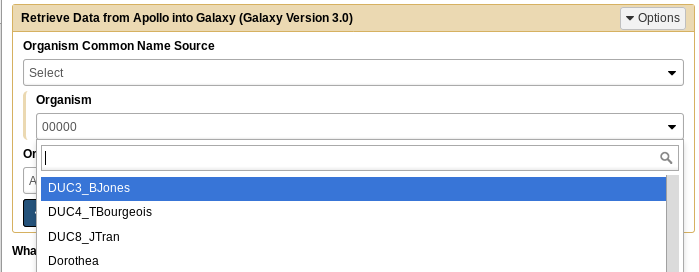
\includegraphics[width=\textwidth]{img/select}
        \end{column}
        \begin{column}{0.38\textwidth}
            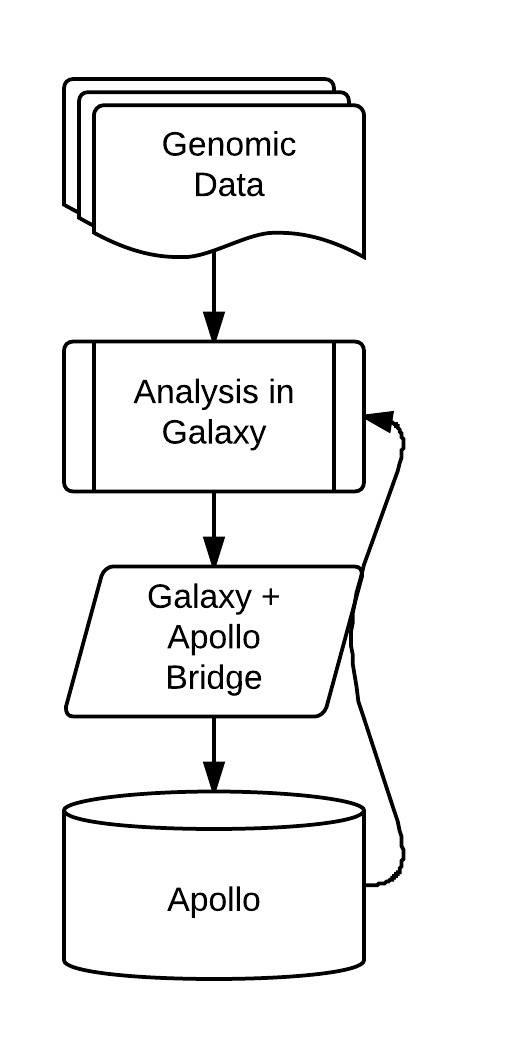
\includegraphics[height=\textheight]{wf.png}
        \end{column}
    \end{columns}
\end{frame}



\section{Databases}

\begin{frame}{Genomic Databases \& Curators}
    \begin{itemize}
        \item Annotator Independence \& Agency
        \item Democratization of resources%. (Easier access control through galaxy tools)
        \item Enabled them to build powerful annotation and analysis pipelines
        \item But also provide appealing UI for annotators
        %\item But how to democratize annotation?
        %\item Galaxy Tools handle CRUD operations \& updating permissions
        %\item (But we do end up having to check user's apollo permissions at every step)
    \end{itemize}
\end{frame}

\subsection{Reproducibility}
\begin{frame}{Reproducibility}
    \begin{itemize}
        \item Reproducibility for generally unreproducible external databases\\
            \begin{equation*}
                \text{Database} = %
                    \textbf{f}_{\text{publication}}(%
                    \textbf{g}_{\text{functional}}(%
                    \textbf{h}_{\text{structural}}(%
                    \text{data}%
                    )))
            \end{equation*}
    \end{itemize}
\end{frame}

\subsection{Tooling}
\begin{frame}{Tooling for Curators}
    \begin{itemize}
        \item Tools for querying annotation resources, answering specific questions. (E.g. Find features with specific qualifier, GO terms)
        \item Tools for fetching data into Galaxy (Chado, Apollo)
        \item Tools for creating new annotations from analysis results
    \end{itemize}
\end{frame}









\section{Teaching}
\begin{frame}{Bacteriophage Annotation Course}
    \begin{itemize}
        \item Undergraduate Phage annotation course
        \item Genome sequence to publication
        \item Parallel track for environmental sample to isolated phage
        \item Novel genome, de novo annotation
        %\item Students run tools in Galaxy, annotate in Apollo, ``published'' data is stored in Chado
        %\item Converging implementations; updates to our phage course + GGA suite
    \end{itemize}
    
\includegraphics[width=4cm]{phage.png}
    
\includegraphics[width=6cm]{pub.png}
\end{frame}

\subsection{Community}
\begin{frame}{Good for Community and Us}
    \begin{itemize}
        \item CPT can leverage the GGA infrastructure
        \item GGA tools help bring community best practices to the CPT
        \item CPT can contribute back well tested workflows
    \end{itemize}
\end{frame}

\subsection{Continuum}
\begin{frame}{Continuum of Community}
    From students to experienced curators: \textbf{collaboration is easy}
    \ \\\ \\
    Supports everyone as they progress

    \begin{itemize}
        \item High level: Apollo is the ``Google Docs'' of genome annotation
        \item Low level: Advanced, custom annotation and analysis pipelines from shared data.
    \end{itemize}
\end{frame}

\section{Future}
\begin{frame}{GGA Going Forward}
    % Too personal to CPT implementation?
    \begin{itemize}
        \item More tools in our Genome Annotation Galaxy Flavour
        \item More tutorials \& training resources
        \item Expand Community
        \item Contribution Fests
    \end{itemize}
    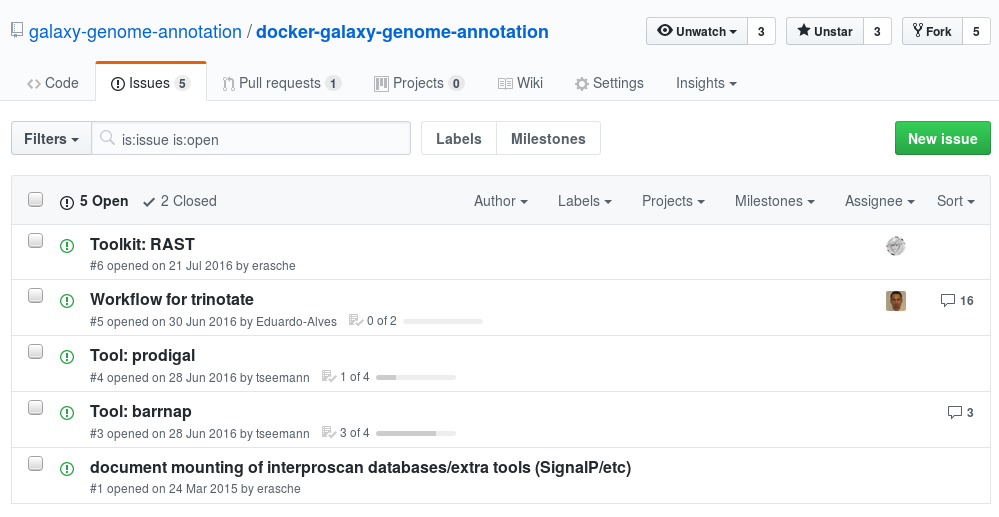
\includegraphics[width=\textwidth]{img/issues}
\end{frame}







\section{Q\&A}
\begin{frame}{Q\&A}
    Thank you and join us at:\\\ \\
    \begin{center}
        \begin{tabular}{ll}
            \color{gray} GGA GitHub & \href{https://galaxy-genome-annotation.github.io/}{galaxy-genome-annotation.github.io}\\
            \color{gray} GGA Gitter & \href{https://gitter.im/galaxy-genome-annotation/Lobby}{gitter.im/galaxy-genome-annotation/Lobby}\\
            \end{tabular}\\[1cm]
            %\logosTamuCPT
            \fundingNSFABIannotation
    \end{center}
\end{frame}

\end{document}
